\documentclass[a4paper, 12pt]{article}

%%%%%%%%%%%%%%%%%%% Packages

%%%%% Tools

\usepackage{comment}
\usepackage{lipsum}
\usepackage{xstring}

%%%%% Document

\usepackage[pdfusetitle]{hyperref}

\usepackage{geometry}
\geometry{paper=a4paper,top=3.5cm,bottom=2.5cm,right=2.5cm,left=2.5cm}

\usepackage{fancyhdr}
\pagestyle{fancy}
\fancyhead[L]{}
\fancyhead[R]{\leftmark}
\fancyfoot[C]{\thepage}
\renewcommand{\headrulewidth}{0pt}

%%%%% Text

\usepackage[utf8]{inputenc}
\usepackage[T1]{fontenc}
\edef\restoreparindent{\parindent=\the\parindent\relax}
\usepackage[parfill]{parskip}
%\restoreparindent
\usepackage{csquotes}

\newlength{\mytextsize}
\makeatletter
\setlength{\mytextsize}{\f@size pt}
\makeatother

%%%%% Languages

\ifx\languages\undefined
	\usepackage[english, french]{babel}
\else
	\usepackage[\languages]{babel}
\fi

% english

\addto\captionsenglish{\def\figurename{Figure}}
\addto\captionsenglish{\def\tablename{Table}}

\newcommand{\st}{\text{s.t.}}

% french

\frenchbsetup{StandardLists=true}

\addto\captionsfrench{\def\figurename{Figure}}
\addto\captionsfrench{\def\tablename{Table}}
\addto\captionsfrench{\def\proofname{Preuve}}

\def\tq{\text{t.q.}}
\def\cad{c.-à-d. }
\def\Cad{C.-à-d. }

%%%%% Styles

\usepackage[skip=\mytextsize]{caption}
\usepackage{float}
\usepackage{mdframed}
\usepackage{enumitem}
\usepackage{eurosym}
\usepackage{color}

\newcommand\caaption[1]{\caption{#1}\vspace{-1\mytextsize}}

%%%%% Mathematics

\usepackage{amsmath}
\usepackage{amssymb}
\usepackage{amsfonts}
\usepackage{bm}
\usepackage{esint}
\usepackage[makeroom]{cancel}

\newcommand{\fact}[1]{#1!}
\newcommand{\e}[1]{\mathbf{e}_{#1}}
\newcommand{\deriv}{\mathrm{d}}
\DeclareMathOperator{\tr}{tr}


%%%%% SI units

\usepackage[squaren,Gray,cdot]{SIunits}
\usepackage{sistyle}

\IfStrEq{\languagename}{french}{
	\SIdecimalsign{,}
}

%%%%% Chemistry

\usepackage[version=4]{mhchem}

%%%%% Table & Figure

\usepackage{array}
\usepackage{tabularx}
\usepackage{multirow}
\usepackage{multicol}
\newcolumntype{M}[1]{>{\centering\arraybackslash}m{#1}}
%\setlength\extrarowheight{0em}
\renewcommand{\arraystretch}{1.3}

\usepackage{pgfplots}
\usepackage{tikz}
\usetikzlibrary{shapes.geometric, positioning}
\usepackage{graphics}
\usepackage{graphicx}
\pgfplotsset{axis on top, compat = 1.3}

%%%%%% Theorems and Definitions

\usepackage{amsthm}
\usepackage{thmtools}

\IfStrEq{\languagename}{english}{
	\def\lgthm{Theorem}
	\def\lglem{Lemma}
	\def\lgprop{Proposition}
	\def\lgdefn{Definition}
	\def\lghyp{Hypothesis}
	\def\lgquest{Question}
	\def\lgansw{Answer}
	\def\lgexpl{Example}
	\def\lgrmk{Remark}
	\def\lgnote{Note}
	\def\lgtip{Tip}
}

\IfStrEq{\languagename}{french}{
	\def\lgthm{Théorème}
	\def\lglem{Lemme}
	\def\lgprop{Proposition}
	\def\lgdefn{Définition}
	\def\lghyp{Hypothèse}
	\def\lgquest{Question}
	\def\lgansw{Réponse}
	\def\lgexpl{Exemple}
	\def\lgrmk{Remarque}
	\def\lgnote{Note}
	\def\lgtip{Conseil}
}

\theoremstyle{plain}
\newtheorem{thm}{\lgthm}[section]
\newtheorem{lem}{\lglem}[section]
\newtheorem{prop}{\lgprop}[section]

\theoremstyle{definition}
\newtheorem{defn}{\lgdefn}[section]
\newtheorem{hyp}{\lghyp}[section]
\newtheorem{quest}{\lgquest}[]

\declaretheorem[
name=\lgansw,
qed={\lower-0.3ex\hbox{$\triangle$}},
within=quest
]{answ}

\declaretheorem[
name=\lgexpl,
qed={\lower-0.3ex\hbox{$\triangle$}},
within=section
]{expl}

\theoremstyle{remark}
\newtheorem*{rmk}{\lgrmk}
\newtheorem*{note}{\lgnote}
\newtheorem*{tip}{\lgtip}

\begingroup
\makeatletter
\@for\theoremstyle:=definition,remark,plain\do{%
	\expandafter\g@addto@macro\csname th@\theoremstyle\endcsname{%
		\addtolength\thm@preskip\parskip
	}%
}
\endgroup

%%%% Others

\renewcommand{\qedsymbol}{$\blacksquare$}

\newcommand{\mytableofcontents}{
	\newpage
	\pagenumbering{roman}
	\tableofcontents
	\newpage
	\pagenumbering{arabic}
}

%%%%%%%%%%%%%%%%%%%

%%%%%%%%%%%%%%%%%%% Titlepage

\def\logopath{include/resources/pdf/logo_uliege.pdf}
\def\toptitle{Université de Liège}
\title{Réseau de régulation génétique}
\def\subtitle{Introduction aux signaux et systèmes}
\author{\textsc{Meurisse} Maxime\\\textsc{Rozet} François\\}
\def\context{2\up{ème} année de Bachelier Ingénieur Civil}
\date{Année académique 2017-2018}

%%%%%%%%%%%%%%%%%%% Others

%%%%%%%%%%%%%%%%%%%

\begin{document}
	\newgeometry{margin = 2.5cm}
\makeatletter
\begin{titlepage}
	\begin{minipage}[t][0.425\textheight][t]{\textwidth}
		\begin{center}
		    \ifx\toptitle\undefined
    		    \vfill
    		    \ifx\logopath\undefined
    		    \else
    			    \includegraphics[height=0.2125\textheight]{\logopath}
    			\fi
    		\else
    		    \ifx\logopath\undefined
    		    \else
    			    \includegraphics[height=0.15\textheight]{\logopath}
    			\fi
    			\vfill
    			{\huge \textsc{\toptitle}}
			\fi
			\vfill
		\end{center}
	\end{minipage}
	\vfill
	\begin{minipage}{\textwidth}
		\hspace{0.5em}
		\begin{mdframed}[linewidth = 2pt, innertopmargin = 1em, innerbottommargin = 1em, leftline = false, rightline = false]
			\begin{center}
				{\huge \bfseries \@title}
			\end{center}
		\end{mdframed}
		\hspace{0.5em}
	\end{minipage}
	\vfill
	\begin{minipage}[b][0.425\textheight][t]{\textwidth}
			\ifx\subtitle\undefined
			\else
			    \vspace{-0.5em}
			    \begin{center}
				    {\LARGE \subtitle}
				\end{center}
			\fi
			\vfill
			\ifx\rightauthor\undefined
			    \begin{center}
			        \ifx\authorhead\undefined
			        \else
		                {\large\it \authorhead\\[0.5em]}
		            \fi
			        {\large \@author}
			    \end{center}
			\else
			    \begin{minipage}[t]{0.5\textwidth}
			        \begin{flushleft}
			            \ifx\authorhead\undefined
			            \else
			                {\large\it \authorhead\\[0.5em]}
			            \fi
				        {\large \@author}
				    \end{flushleft}
				\end{minipage}
				\begin{minipage}[t]{0.5\textwidth}
				    \begin{flushright}
				        \ifx\rightauthorhead\undefined
			            \else
			                {\large\it \rightauthorhead\\[0.5em]}
			            \fi
				        {\large \rightauthor}
				    \end{flushright}
				\end{minipage}
			\fi
			\vfill
			\begin{center}
			    \ifx\context\undefined
			    \else
			        {\large \context \\[0.5em]}
			    \fi
			    {\large \@date}
			\end{center}
	\end{minipage}
\end{titlepage}
\makeatother
\restoregeometry
	\section{Expression constitutive de gènes}
	\subsection{Influence des paramètres ${k}_{1}$, ${k}_{2}$, ${d}_{1}$ et ${d}_{2}$}
	Intuitivement, les paramètres ${d}_{i}$ décrivent la réactivité du système. Plus ils sont élevés, plus le système réagira rapidement à l'entrée. Notamment, s'ils sont très élevés, la sortie tendra vers un multiple de l'entrée (déterminé par les paramètres ${k}_{i}$).
	\subsection{Entrée(s), sortie(s) et état(s) du système}
	Toutes les variables de ce système sont définies à partir du temps $t = 0$, \cad lorsque commence la transcription de l'ADN en mRNA.
	L’entrée de ce système est $g$, la concentration en gènes.
	La sortie de ce système est $p$, la concentration en protéines.
	Les états de ce système sont $m$, la concentration en mRNA et $p$.
	Une concentration est toujours un réel positif.
	\begin{table}[H]
		\centering
		\begin{tabular}{| c | c | c | c |}
			\hline
			\textbf{Variable d'état} & \textbf{Variable} & \textbf{Domaine} & \textbf{Image}\\
			\hline
			\hline
			Entrée & $g$ & $\mathbb{R}^{+}$ & $\mathbb{R}^{+}$\\
			\hline
			Sortie & \multirow{2}{*}{$p$} & \multirow{2}{*}{$\mathbb{R}^{+}$} & \multirow{2}{*}{$\mathbb{R}^{+}$}\\
			\cline{1-1}
			\multirow{2}{*}{\'{E}tats} &&&\\
			\cline{2-4}
			& $m$ & $\mathbb{R}^{+}$ & $\mathbb{R}^{+}$\\
			\hline
		\end{tabular}
		\caption{Variables d'état du système}
	\end{table}
	\subsection{Type du système}
	Le système d'équations différentielles proposé est composé d'équations différentielles linéaires à coefficients constants. Il est donc linéaire et temps-invariant, alias LTI.
	\subsubsection{Le(s) point(s) d'équilibre(s)}
	Le système sera à l'équilibre lorsque, pour une entrée constante, les états et la sortie seront constants, \cad lorsque $\dot{m}$ et $\dot{p}$ seront nuls.
	\begin{equation}
		\left\{
		\begin{aligned}
			{d}_{1}m & = {k}_{1}g \\
			{d}_{2}p & = {k}_{2}m
		\end{aligned}
		\right.
	\end{equation}
	\subsection{Représentation d'état}
	En représentant l'entrée $g$ du système par $u$ et la sortie $p$ du système par $y$, on obtient la représentation d'état :
	\begin{equation}
		\left\{
		\begin{aligned}
			\dot{\bm x} & = A \cdot {\bm x} + B \cdot u \\
			y           & = C \cdot {\bm x} + D \cdot u
		\end{aligned}
		\right.
	\end{equation}
	Avec
	\begin{align}
		A & = 
		\begin{pmatrix}
			-{d}_{1} & 0        \\
			{k}_{2}  & -{d}_{2}
		\end{pmatrix} &
		B & = 
		\begin{pmatrix}
			{k}_{1} \\
			0
		\end{pmatrix} &
		C & =
		\begin{pmatrix}
			0 & 1
		\end{pmatrix} &
		D & =
		\begin{pmatrix}
			0
		\end{pmatrix}
	\end{align}
	\subsection{Critère de stabilité}
	Le système est stable si les valeurs propres de sa matrice $A$ sont strictement négatives.
	\begin{alignat*}{2}
		                      &  & 0 & = \left|A-\mathbb{I}_2\lambda\right|                       \\
		\Leftrightarrow \quad &  & 0 & = 
		\begin{vmatrix}
		-{d}_{1}-\lambda & 0                \\
		{k}_{2}          & -{d}_{2}-\lambda
		\end{vmatrix} \\
		\Leftrightarrow \quad &  & 0 & = \left({d}_{1}+\lambda\right)\left({d}_{2}+\lambda\right)
	\end{alignat*}
	Les valeurs propres sont $-{d}_{1}$ et $-{d}_{2}$ et sont strictement négatives si ${d}_{1}$ et ${d}_{2}$ sont strictement positifs.
	\subsection{Réponse libre du système}
	Grâce aux valeurs propres calculées et puisque le système est LTI, on peut écrire la réponse libre du système comme :
	\begin{align}
		y(t) & = {m}_{0}e^{-{d}_{1}t} + {p}_{0}e^{-{d}_{2}t}
	\end{align}
	Avec ${m}_{0}$ et ${p}_{0}$, respectivement, les valeurs initiales des variables $m$ et $p$.\\
	Dès lors, à partir de l'énoncé, on trouve :
	\begin{align}
		{d}_{1} & = \frac{1}{{\tau}_{m}} & \text{ et } && {d}_{2} & = \frac{1}{{\tau}_{p}}
	\end{align}
	\subsection{Réponses du système}
	Les réponses obtenues ont été calculées pour des conditions initiales nulles ($m$ et $p = 0$).
	\subsubsection{Réponse impulsionnelle}
	La réponse impulsionnelle est la réponse d'un système à une impulsion de Dirac.\\
	Plusieurs bonnes approximations de cette impulsion existent. On a choisi celle-ci, appelée impulsion gaussienne :
	\begin{align}
		\delta(t) & = \lim\limits_{a \rightarrow 0} \frac{{e}^{-\left(\frac{x}{a}\right)^{2}}}{a\sqrt{2\pi}}
	\end{align}
	Pour $a$ valant $\num{2e-2}$, on obtient comme réponse impulsionnelle :
	\begin{figure}[H]
		\centering
		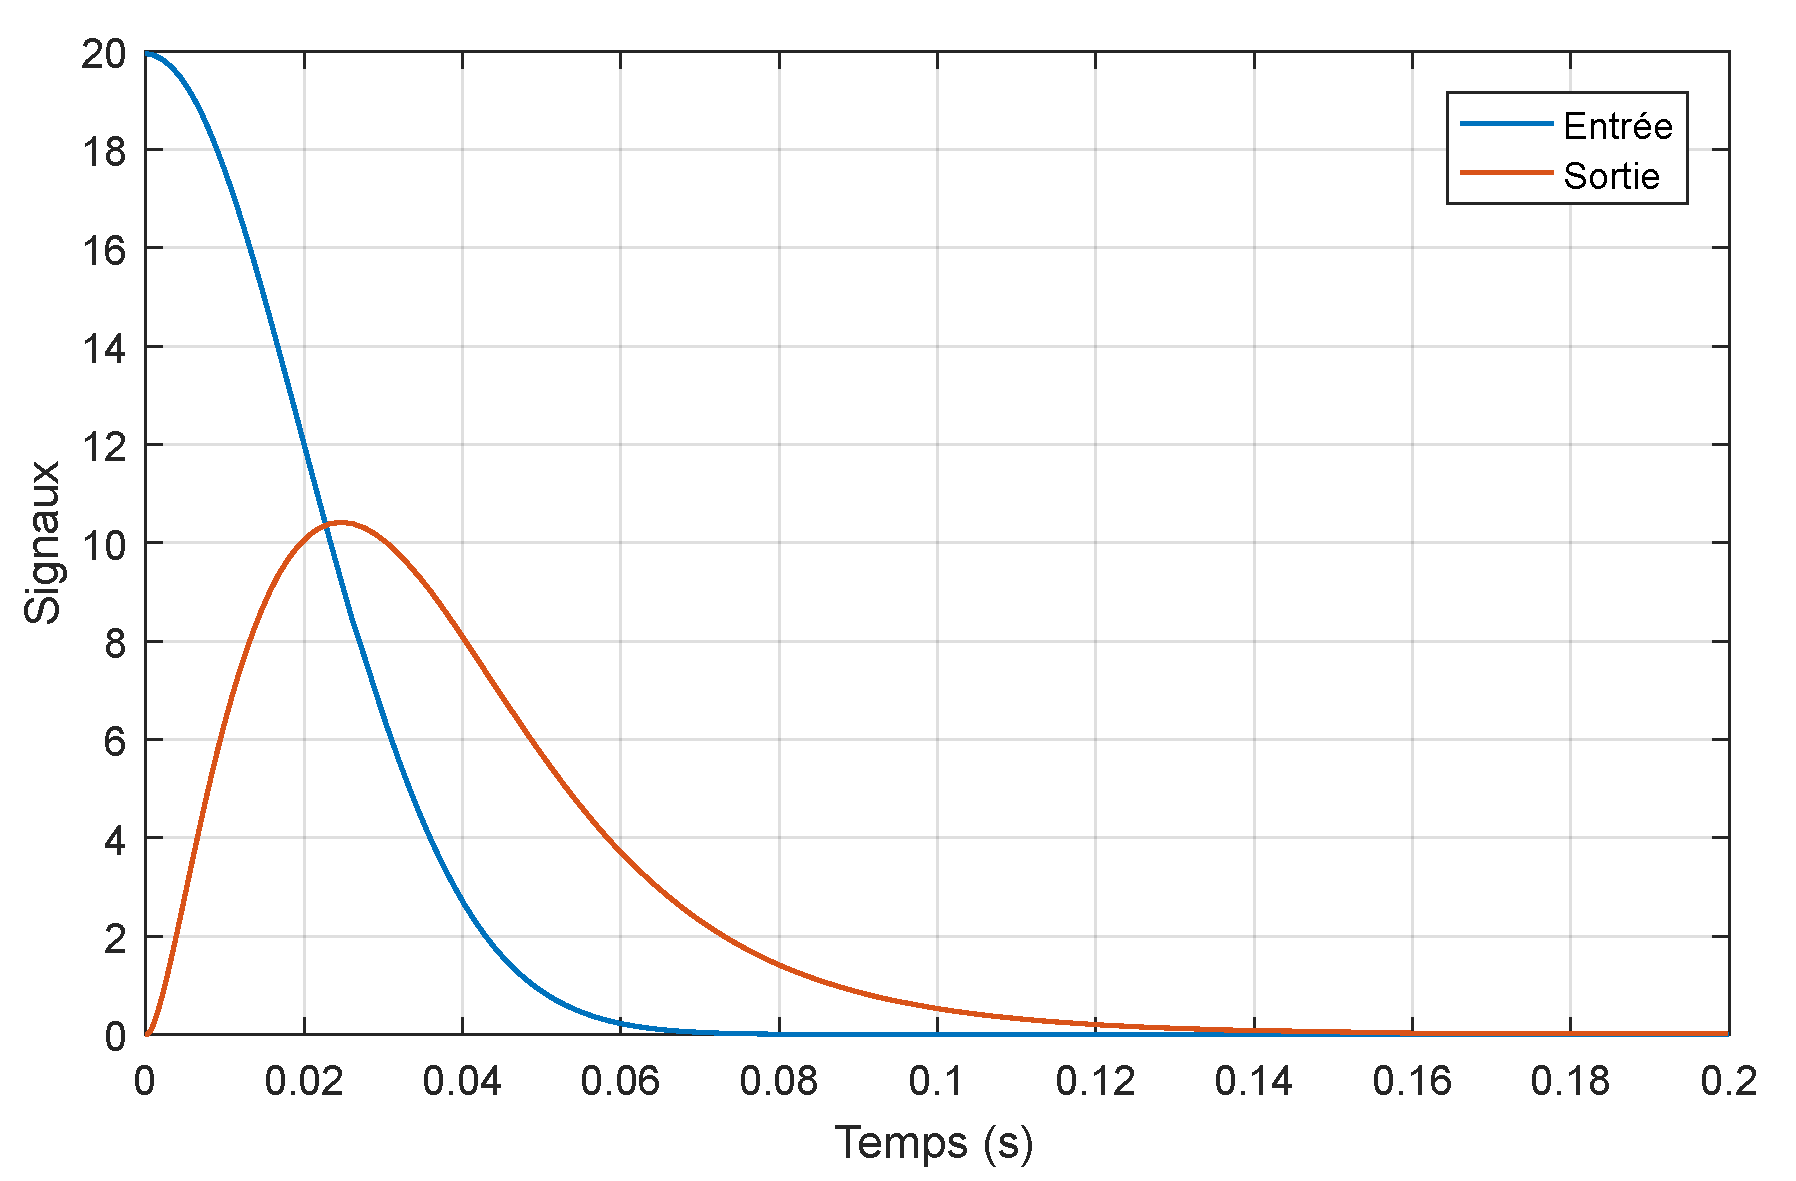
\includegraphics[width = 0.65\textwidth]{resources/pdf/rep_imp.pdf}
		\caption{Réponse impulsionnelle du système}
	\end{figure}
	En effectuant plusieurs tests, on remarquera que plus l'impulsion est brusque, \cad plus $a$ est proche de $0$, moins la sortie du système est proche de l'entrée.\\
	\subsubsection{Réponse indicielle}
	La réponse indicielle est la réponse d'un système à un échelon unitaire. \\
	\begin{comment}
	La définition de cet échelon est :
	\begin{align}
		\sigma(t) = 
		\begin{cases}
			0 & \text{pour } t < 0    \\
			1 & \text{pour } t \geq 0
		\end{cases}
	\end{align}
	\end{comment}
	\begin{figure}[H]
		\centering
		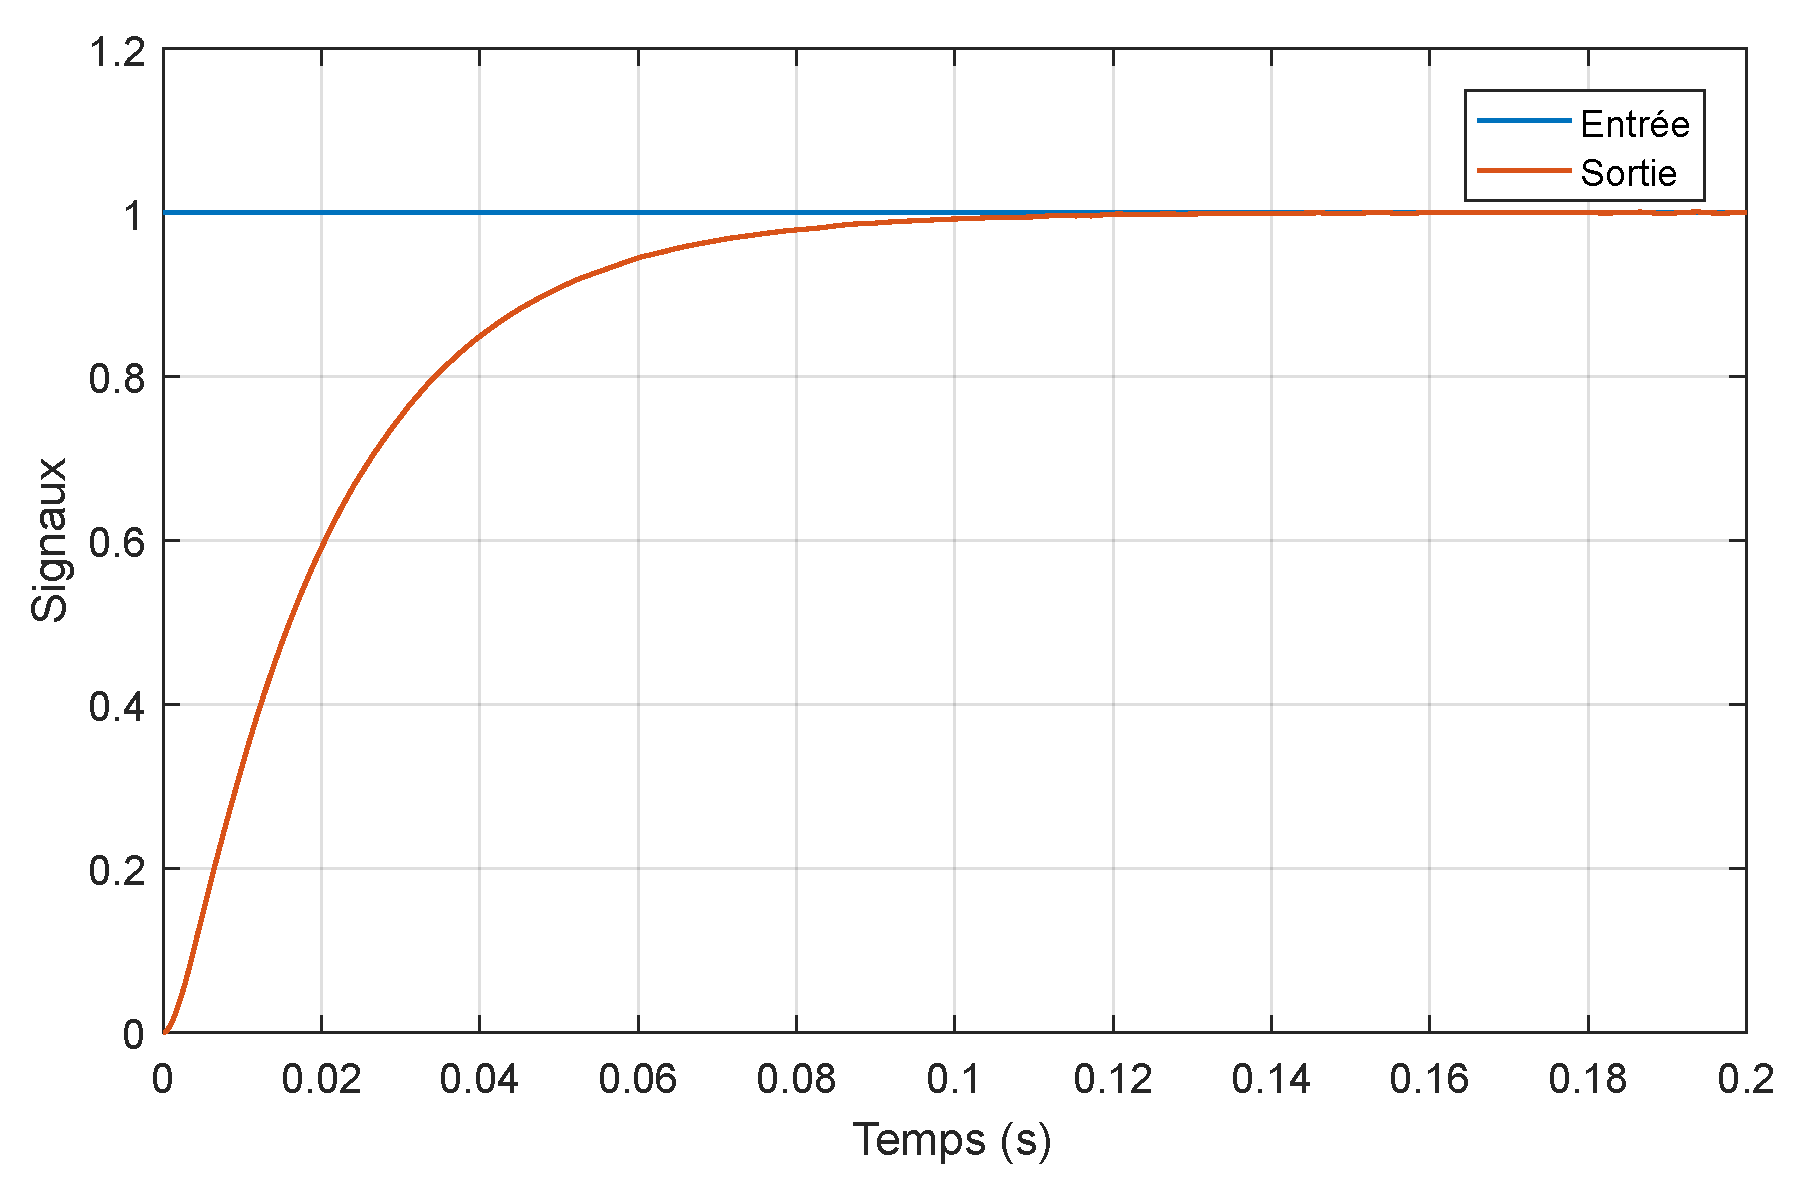
\includegraphics[width = 0.65\textwidth]{resources/pdf/rep_ind.pdf}
		\caption{Réponse indicielle du système}
	\end{figure}
	\subsection{Discussion des effets des différents paramètres}
	D'après l'expression de la réponse libre, on constate que seuls les paramètres ${d}_{i}$ affectent les temps de réponses. Une diminution d'un ${d}_{i}$ entrainera une augmentation de réactivité du système, affectant sa dynamique.\\
	Les facteurs ${k}_{1}$ et ${k}_{2}$ sont, quant à eux, des facteurs influençant les \og{} quantités \fg{} produites. Par exemple, ils peuvent modifier l'amplitude d'un maximum de la sortie mais ils ne modifieront pas sa position au cours du temps. Ils affectent donc uniquement les propriétés statiques du système.
	\begin{figure}[H]
		\centering
		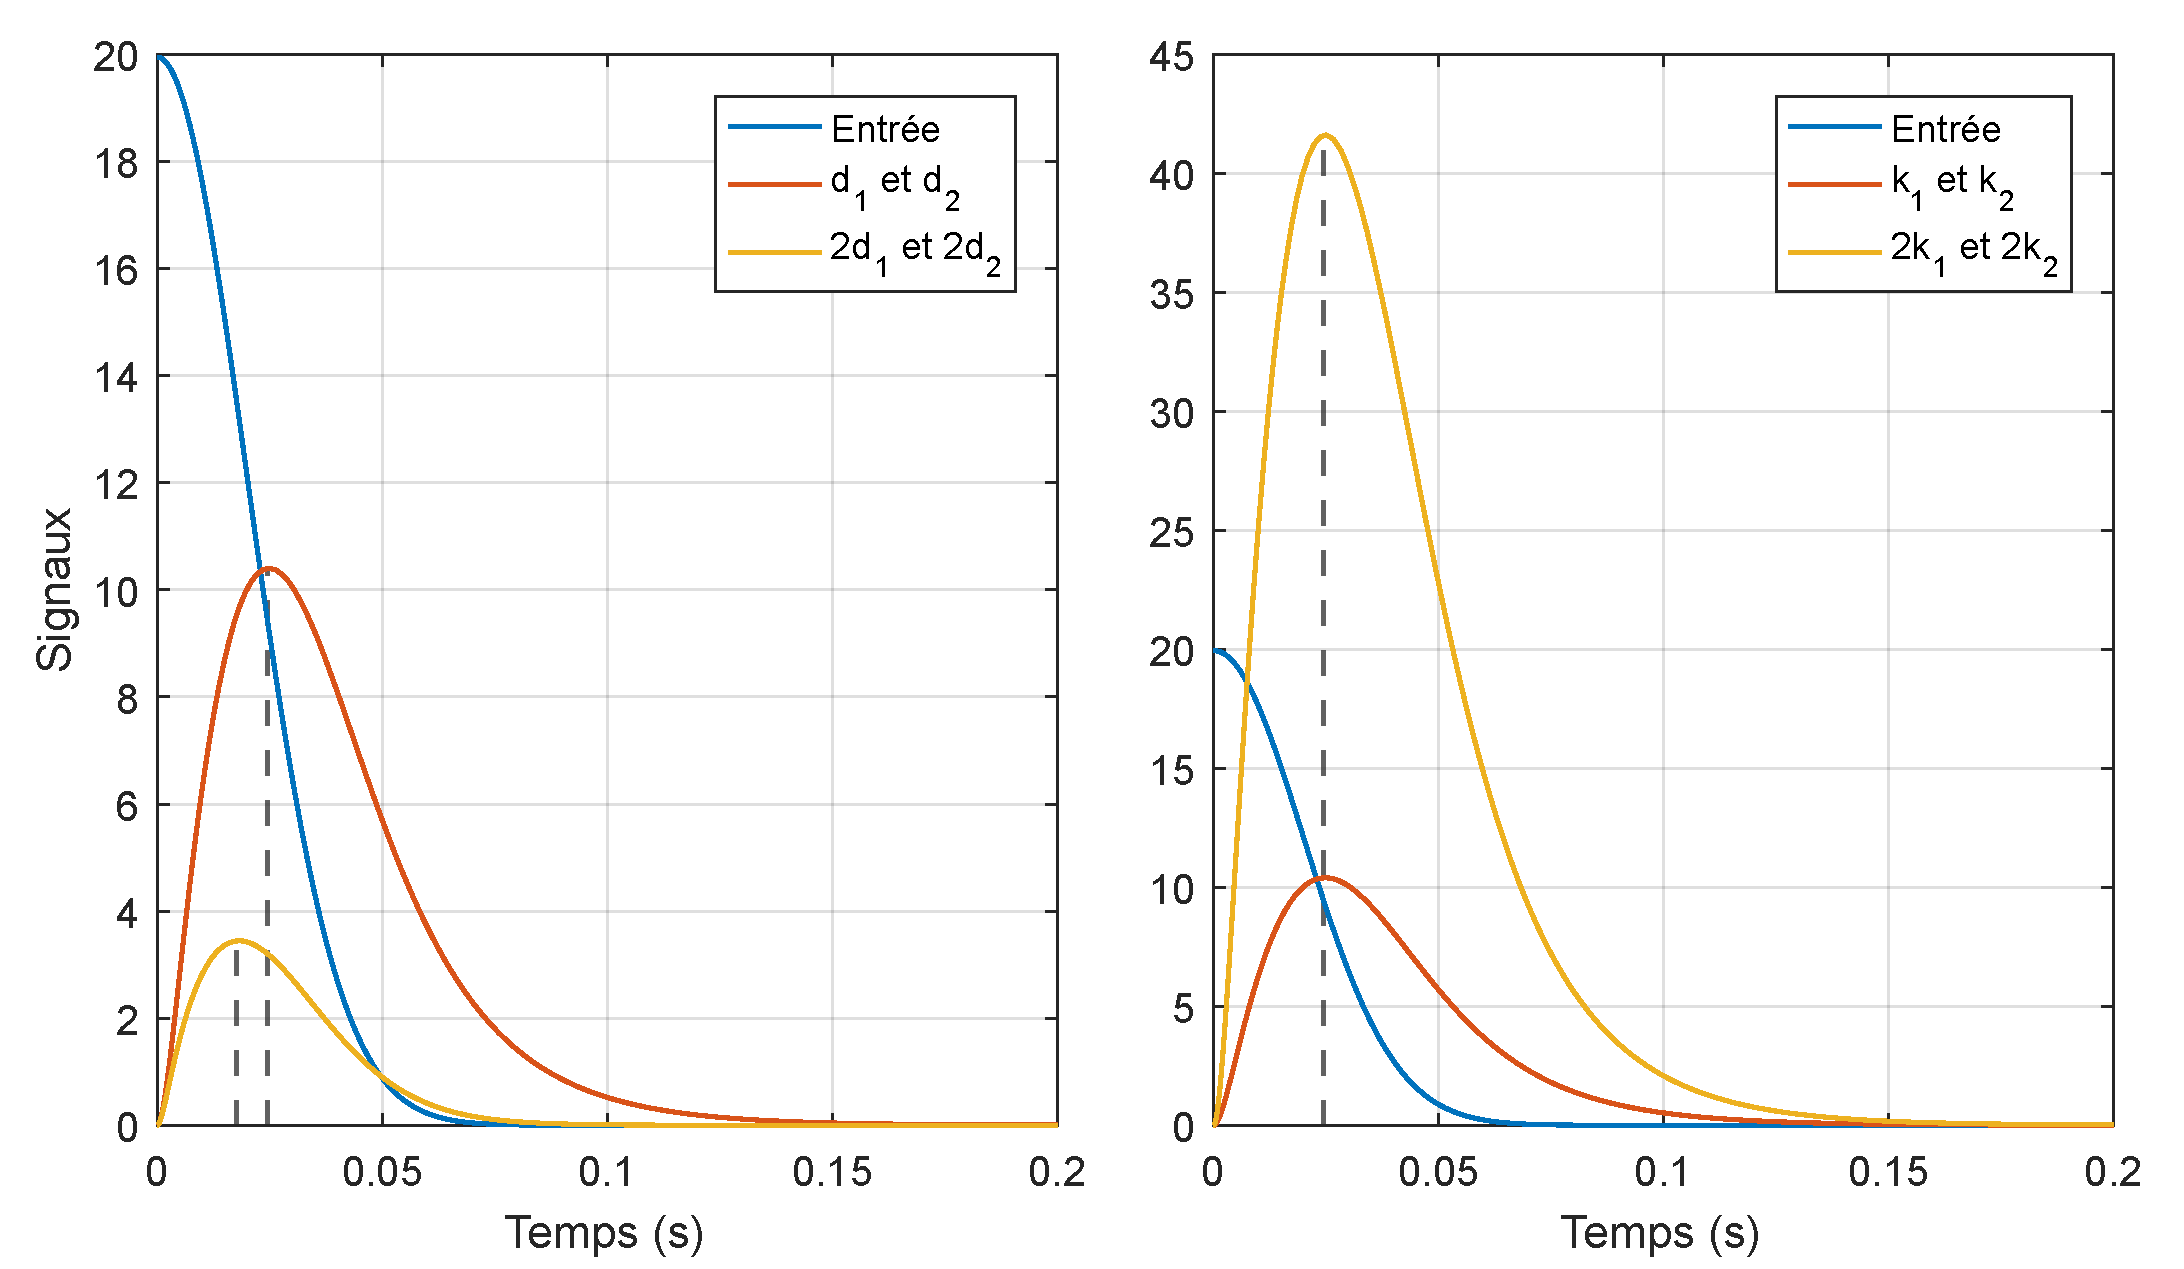
\includegraphics[width = 0.85\textwidth]{resources/pdf/effet_param.pdf}
		\caption{Simulations illustrant les effets des différents paramètres}
	\end{figure}
	\subsection{Réponse du système à des entrées cosinus}
	On doit soumettre le système à une entrée cosinus de pulsation variable.
	\begin{align}
		u(t) & = \cos \left(\omega t\right) 
	\end{align}
	Avec $\omega$, la pulsation. \\
	En soumettant le système à cette entrée, on obtient comme réponse :
	\begin{figure}[H]
		\centering
		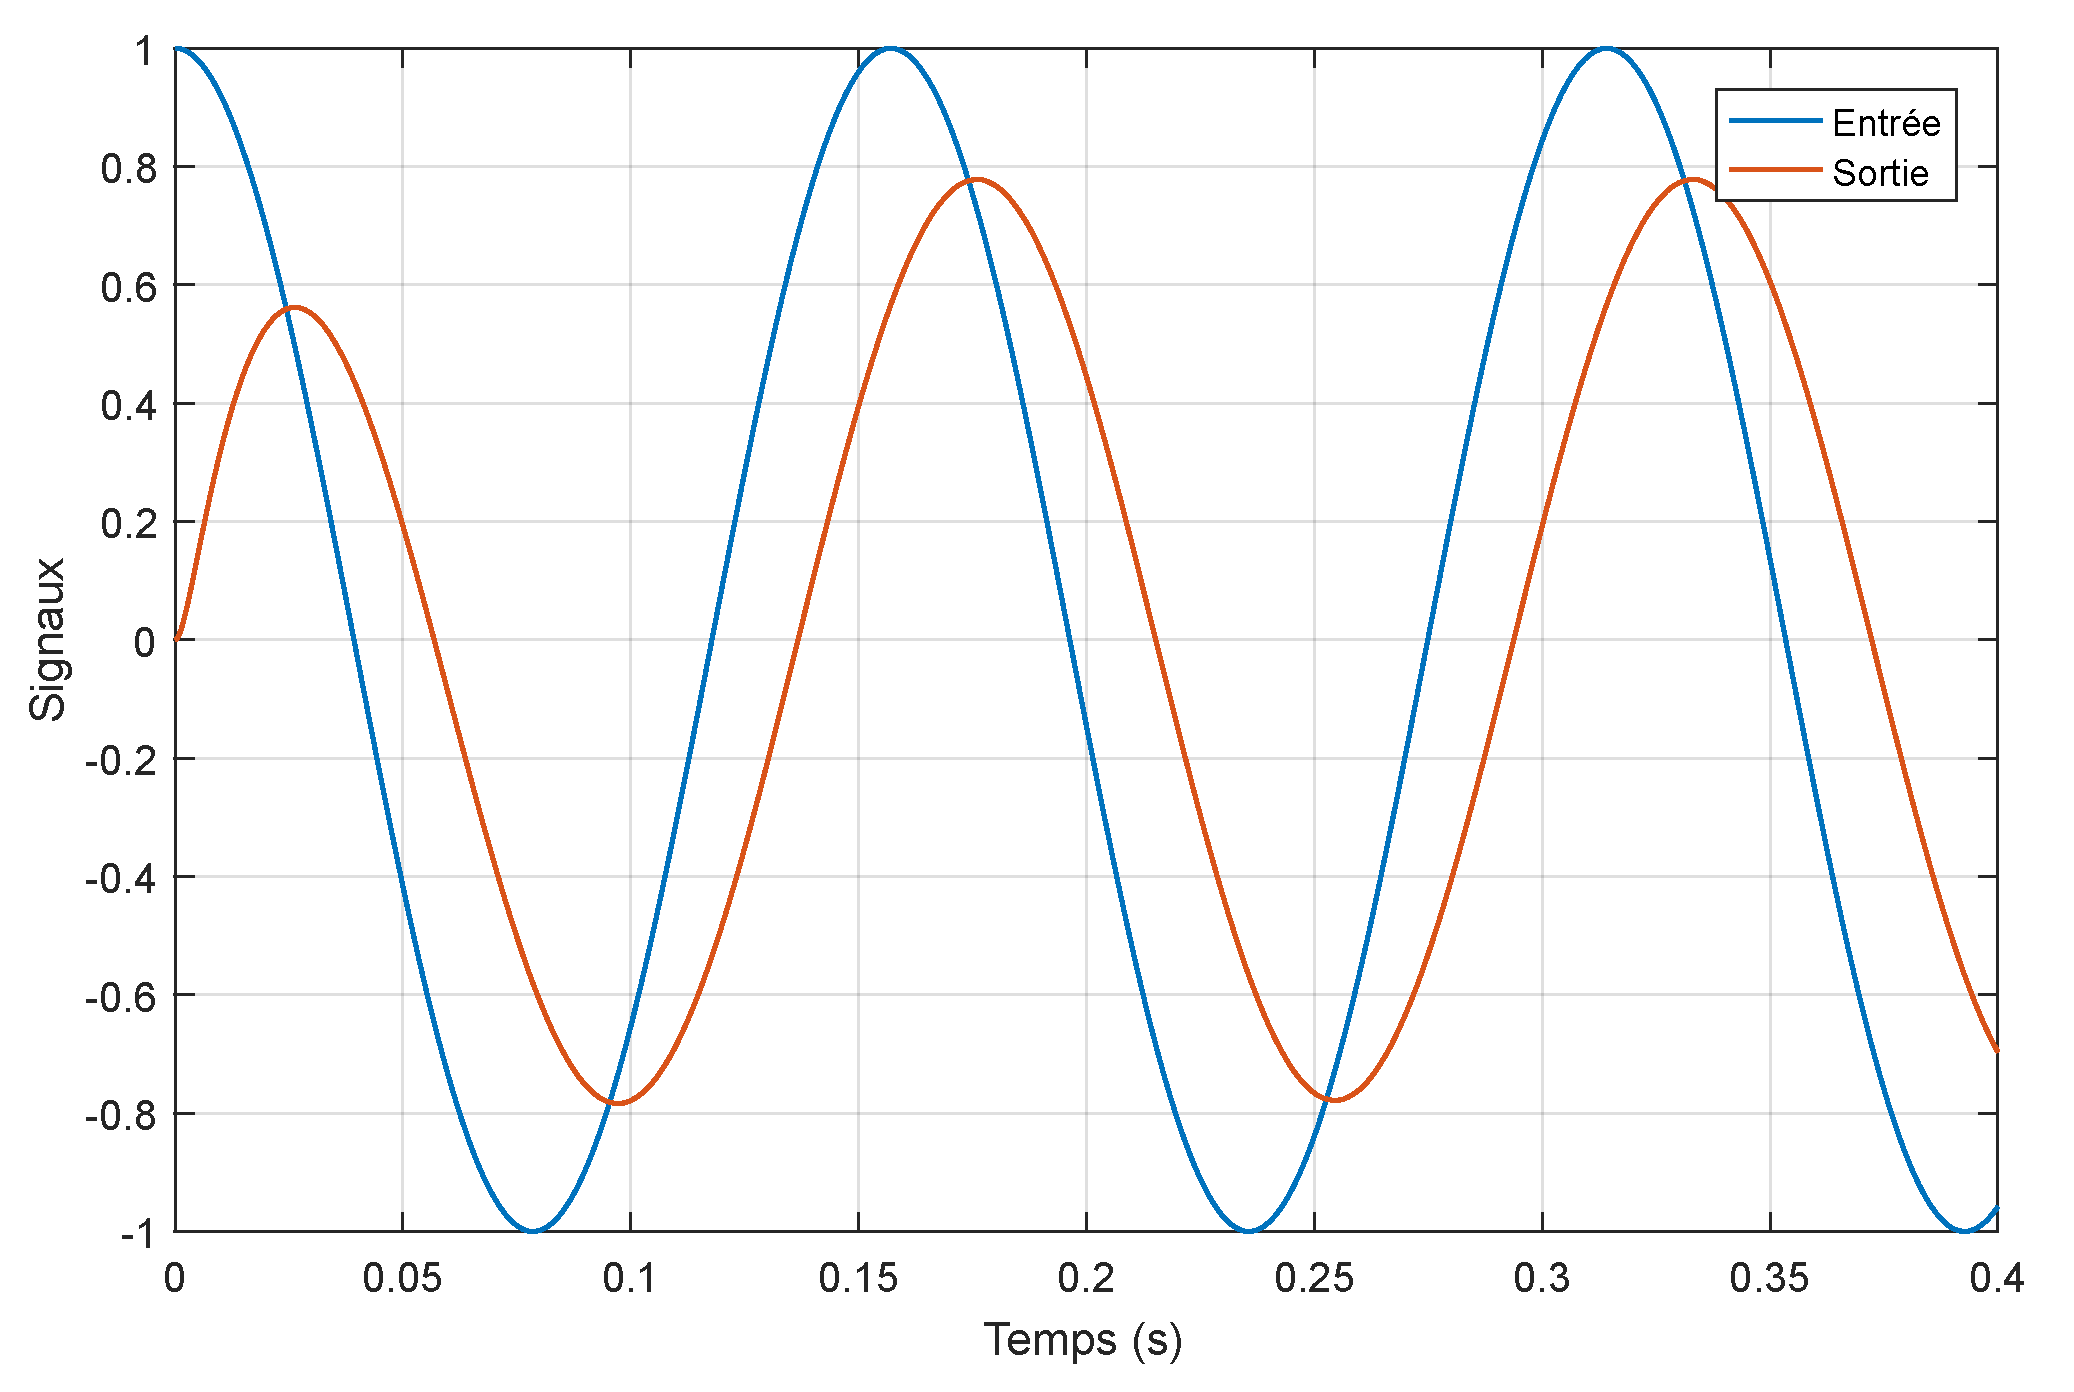
\includegraphics[width = 0.65\textwidth]{resources/pdf/rep_cos.pdf}
		\caption{Réponse du système pour une entrée cosinus de pulsation $\unit{40}{\rad\usk\hertz}$}
	\end{figure}
	On remarque, en comparant pour différentes valeurs de $\omega$, que, à partir d'une pulsation de $\unit{10}{\rad\usk\hertz}$, plus elle est élevée, plus la sortie perd en amplitude et plus elle est déphasée (négativement). On peut qualifier ce comportement de passe-bas.
	\begin{comment}
	\subsection{Fonction de transfert et diagrammes de Bode}
	\textsc{MATLAB} permet de calculer numériquement la fonction de transfert d'un système. En utilisant ces fonctionnalités, on obtient :
	\begin{align}
		\texttt{tf(ss(A, B, C, D))} & = \frac{25000}{{s}^{2} + 550 s + 25000}                                                  \\
		                            & = \frac{{k}_{1} {k}_{2}}{{s}^{2} + \left({d}_{1} + {d}_{2}\right) {s} + {d}_{1} {d}_{2}} \\
		                            & = \frac{{k}_{1} {k}_{2}}{\left(s + {d}_{1}\right)\left(s + {d}_{2}\right)}
	\end{align}
	Il permet aussi, à partir d'une fonction de transfert, de tracer les diagrammes de Bode.
	\begin{figure}[H]
		\centering
		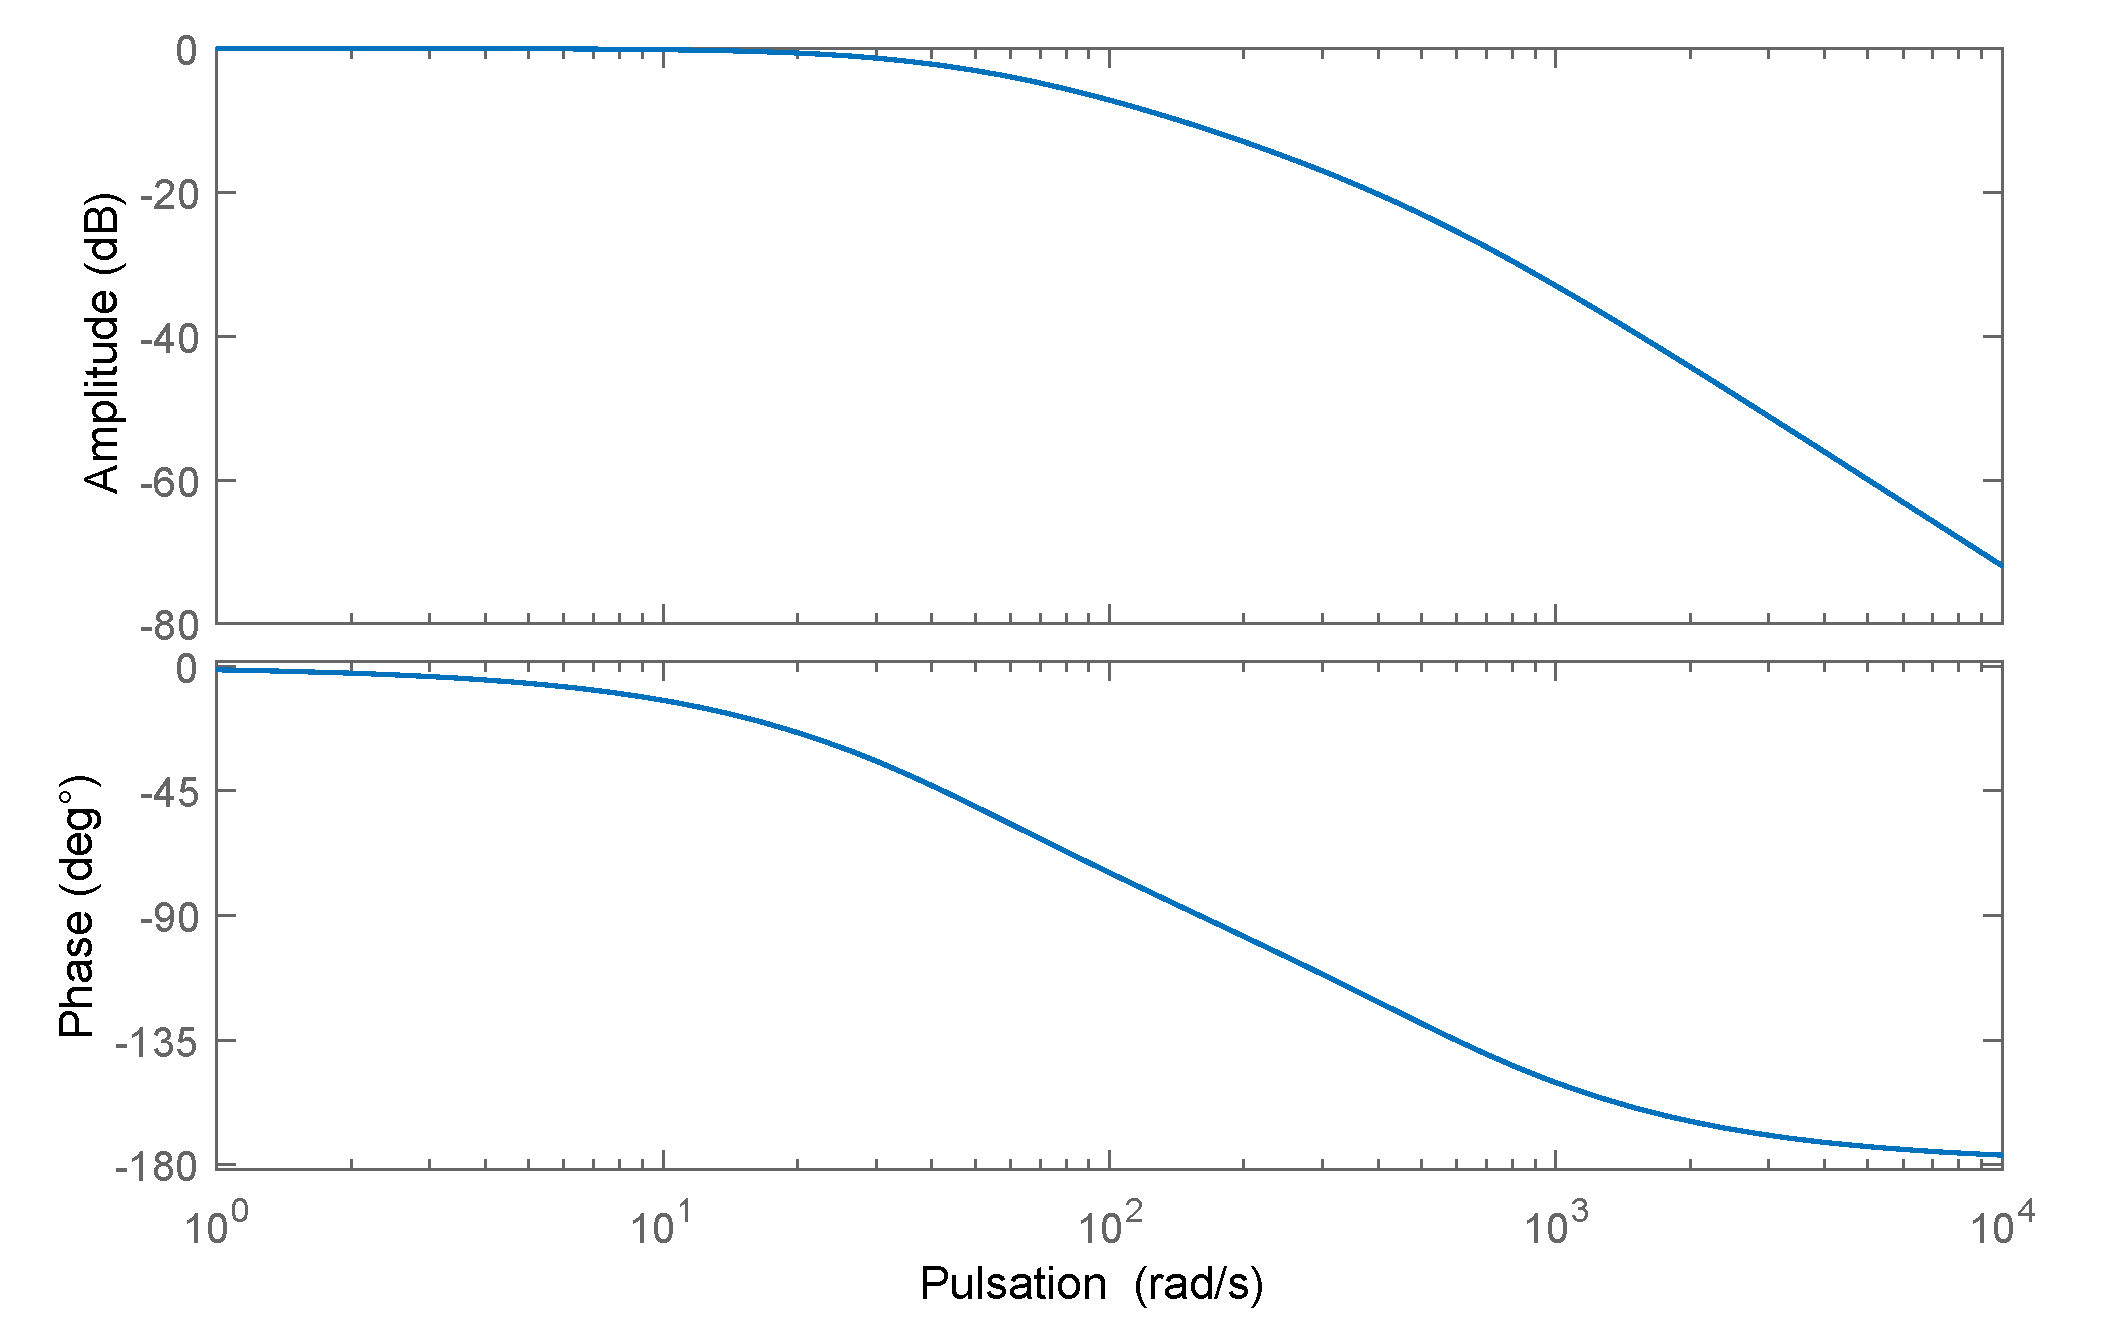
\includegraphics[width = 0.65\textwidth]{resources/pdf/bode.pdf}
		\caption{Diagrammes de Bode calculés numériquement}
	\end{figure}
	En observant ces diagrammes, on note que, en accord avec les conclusions posées au point précédent, la sortie voit son amplitude décroitre et sa phase diminuer pour des $\omega$ élevés. Le déphasage maximal, $\unit{-\pi}{\rad}$, est atteint à une pulsation $\unit{\num{e4}}{\rad\usk\hertz}$ alors que l'amplitude, elle, garde toujours une pente décroissante de $\unit{40}{\deci\bel}$ par décades après $\unit{\num{e3}}{\rad\usk\hertz}$.
	\subsubsection{Calcul analytique de la fonction de transfert}
	Transformons le système donné :
	\begin{align*}
	&
	\left\{\begin{aligned}
		\dot{m} & = {k}_{1}u - {d}_{1}m \\
		\dot{y} & = {k}_{2}m - {d}_{2}y
	\end{aligned}\right. \\
	\Rightarrow \quad &
	\left\{\begin{aligned}
		\dot{m}  & = {k}_{1}u - {d}_{1}m             \\
		\dot{y}  & = {k}_{2}m - {d}_{2}y             \\
		\ddot{y} & = {k}_{2}\dot{m} - {d}_{2}\dot{y}
	\end{aligned}\right. \\
	\Leftrightarrow \quad &
	\left\{\begin{aligned}
		\dot{m} & = & {k}_{1}u - {d}_{1}m                                          \\
		m       & = & \frac{{d}_{2}}{{k}_{2}}y + \frac{1}{{k}_{2}}\dot{y}        \\
		\dot{m} & = & \frac{{d}_{2}}{{k}_{2}}\dot{y} + \frac{1}{{k}_{2}}\ddot{y}
	\end{aligned}\right.
	\end{align*}
	Ainsi,
	\begin{alignat}{2}
		                                             &  & \frac{{d}_{2}}{{k}_{2}}\dot{y} + \frac{1}{{k}_{2}}\ddot{y}                  & = {k}_{1}u - {d}_{1} \left(\frac{{d}_{2}}{{k}_{2}}y + \frac{1}{{k}_{2}}\dot{y}\right) \nonumber \\
		\Leftrightarrow \quad                        &  & \ddot{y} + \left({d}_{1} + {d}_{2}\right) \dot{y} + {d}_{1} {d}_{2} y       & = {k}_{1} {k}_{2} u \nonumber                                                                   \\
		\overset{\mathcal{L}}{\longrightarrow} \quad &  & {s}^{2}Y(s) + \left({d}_{1} + {d}_{2}\right) {s}Y(s) + {d}_{1} {d}_{2} Y(s) & = {k}_{1} {k}_{2} U(s)
	\end{alignat}
	Il est maintenant possible de calculer la fonction de transfert :
	\begin{align}
		H(s) & = \frac{Y(s)}{U(s)} \nonumber                                                                      \\
		     & = \frac{{k}_{1} {k}_{2}}{{s}^{2} + \left({d}_{1} + {d}_{2}\right) {s} + {d}_{1} {d}_{2}} \nonumber \\
		     & = \frac{{k}_{1} {k}_{2}}{\left(s + {d}_{1}\right)\left(s + {d}_{2}\right)}
	\end{align}
	\subsubsection{Régions de convergence}
	Considérons ${\sigma}_{min}$ et ${\sigma}_{max}$ les parties réelles, respectivement, la plus petite et la plus grande des pôles de convergence de $H(s)$ ($-{d}_{2}$ et $-{d}_{1}$).
	On peut noter les deux régions de convergence :
	\begin{alignat*}{2}
		\text{Causal : }      &  & s \in \mathbb{C} \text{: } & \mathbb{R}(s) > {\sigma}_{max} \\
		\text{Anti-causal : } &  & s \in \mathbb{C} \text{: } & \mathbb{R}(s) < {\sigma}_{min}
	\end{alignat*}
	${d}_{1}$ étant positif, la région de convergence pour laquelle le système est causal, est aussi BIBO stable.
	\subsubsection{Diagrammes de Bode}
	\begin{align*}
		H(s) & = \frac{{k}_{1} {k}_{2}}{{d}_{2} - {d}_{1}}\frac{1}{\left(s + {d}_{1}\right)} + \frac{{k}_{1} {k}_{2}}{{d}_{1} - {d}_{2}}\frac{1}{\left(s + {d}_{2}\right)}
	\end{align*}
	\end{comment}
	\section{Expression de gènes avec auto-activation}
	\subsection{Modification du système d'équations}
	Ce qui stimulait, auparavant, la production de protéines était $g$, la concentration en gènes. Ce qui stimule, maintenant, la production est $f(p)$, l'auto-activation dépendant de la concentration en protéines.
	\begin{align}
		\left\{
		\begin{aligned}
			\dot{m} & = {k}_{1}{f}(p) - {d}_{1}m \\
			\dot{p} & = {k}_{2}m - {d}_{2}p
		\end{aligned}
		\right.
	\end{align}
	\subsection{Type du système}
	Le système d'équations différentielles proposé est composé d'équations différentielles non-linéaires à coefficients constants. Il est donc non-linéaire et temps-invariant.
	\subsubsection{Le(s) point(s) d'équilibre(s)}
	Ne dépendant pas de l'entrée, le système sera à l'équilibre lorsque, indépendamment de l'entrée, les états et la sortie seront constants, \cad lorsque $\dot{m}$ et $\dot{p}$ seront nuls.
	\begin{align}
		\left\{
		\begin{aligned}
			0 & = {k}_{1}\left(1 - \frac{{K}^{n}}{{K}^{n} + {p}^{n}}\right) - {d}_{1}m \\
			0 & = {k}_{2}m - {d}_{2}p
		\end{aligned}
		\right.
	\end{align}
	Ce système admet $n + 1$ solutions. La valeur de $n$, dans ce cas, étant $5$, il en possède $6$. En utilisant la condition donnée ${d}_{i} = {k}_{i}$ :
	\begin{figure}[H]
		\centering
		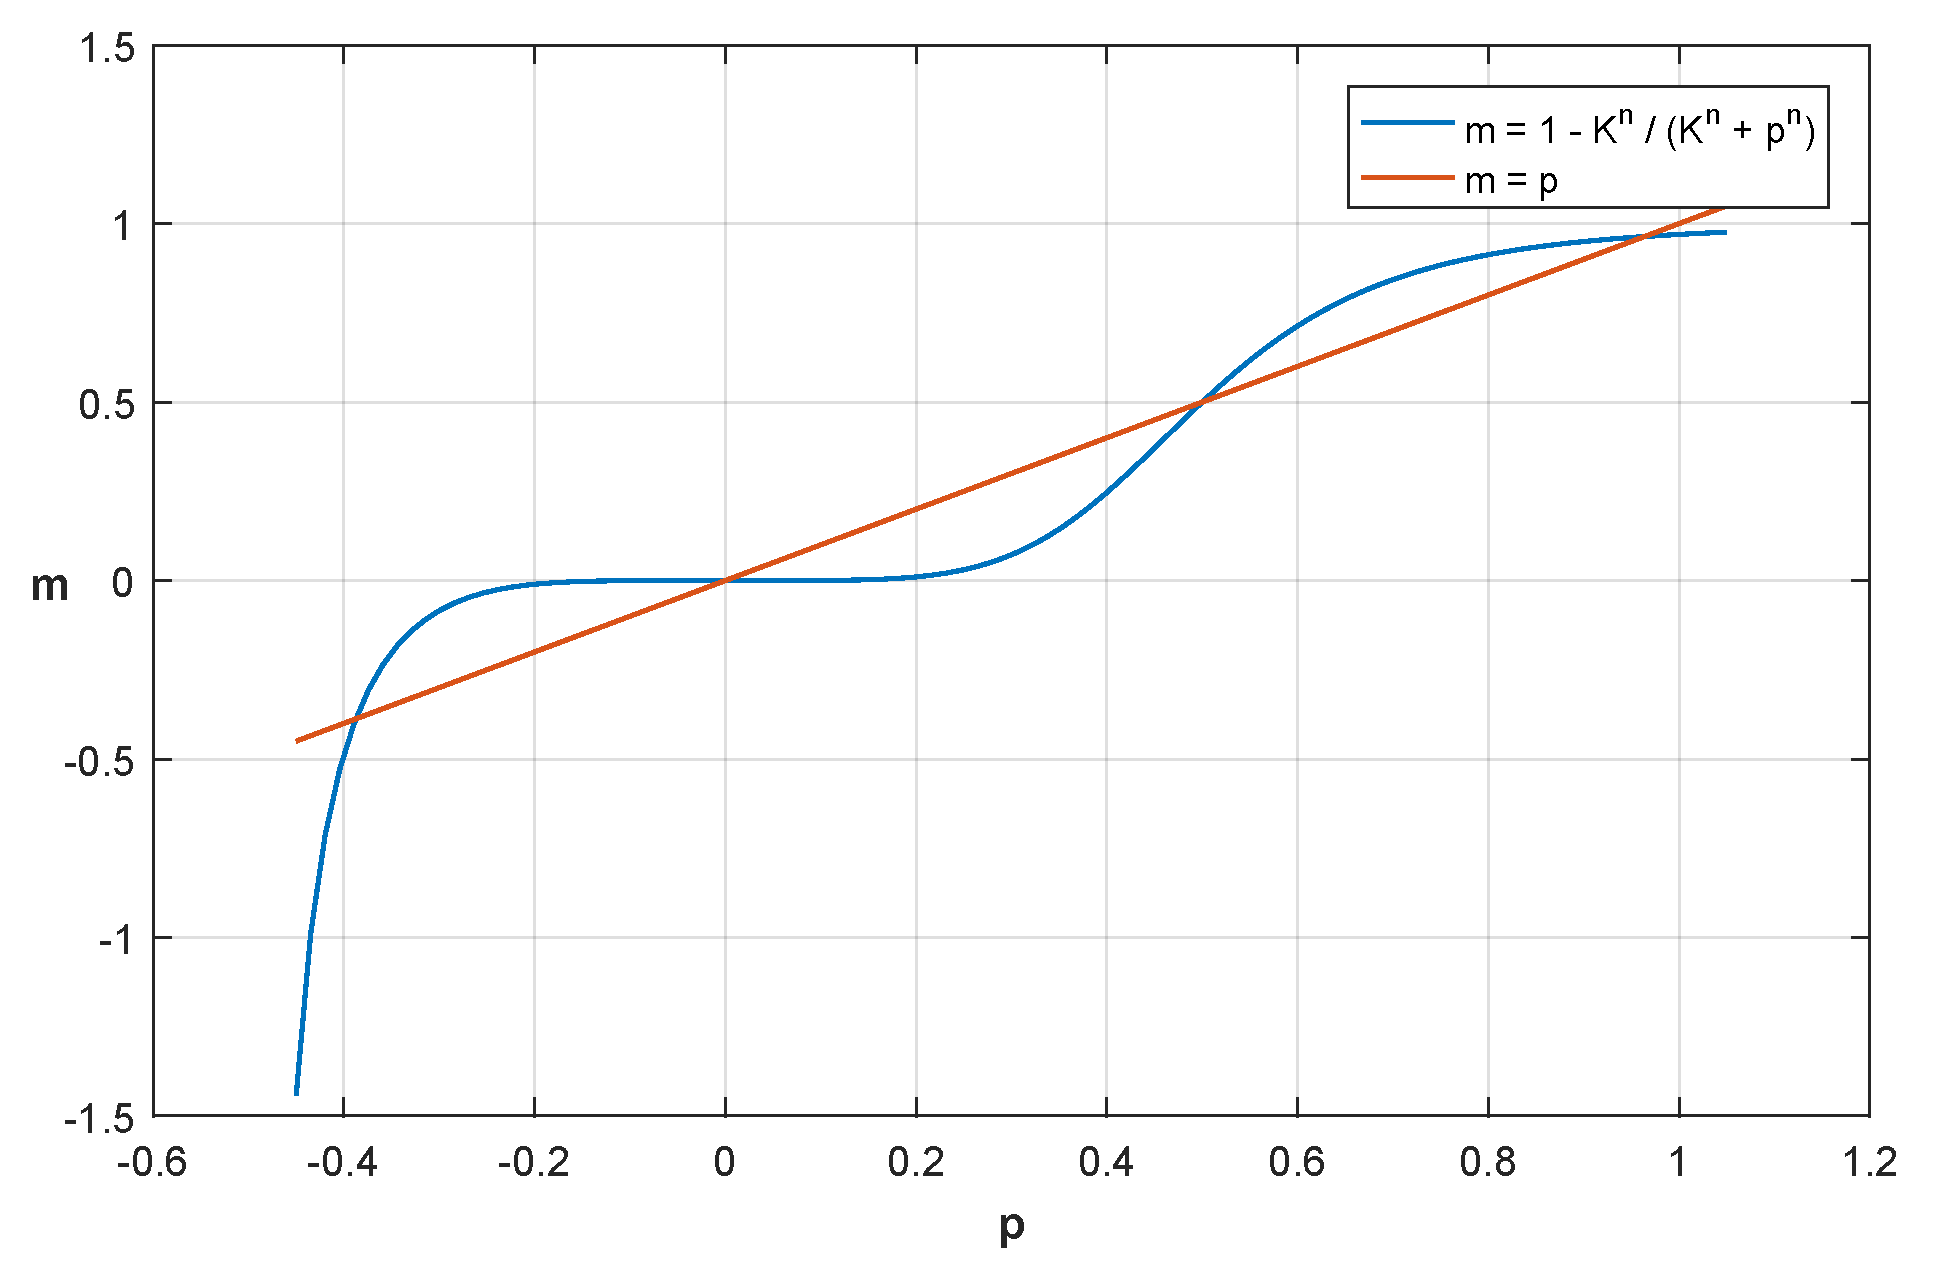
\includegraphics[width = 0.65\textwidth]{resources/pdf/m2p.pdf}
		\caption{Les points d'équilibres}
	\end{figure}
	Graphiquement, on en observe seulement $4$. Numériquement, les points d'équilibres obtenus sont :
	\begin{align*}
		p = m & = 
		\begin{bmatrix}
			0.964 & \frac{1}{2} & 0 & -0.387  & -0.038 - 0.407i & -0.038 + 0.407i
		\end{bmatrix}
	\end{align*}
	Les concentrations $p$ et $m$ étant réelles et positives, on ne sélectionne que les trois premiers points d'équilibre.
	\subsection{Stabilité des points d'équilibre}
	En linéarisant autour des points d'équilibre, on obtient le système
	\begin{align}
		\left\{
		\begin{aligned}
			\dot{\bar{m}} & = {d}_{1}{f'}({p}^{*})\bar{p} - {d}_{1}\bar{m} \\
			\dot{\bar{p}} & = {d}_{2}\bar{m} - {d}_{2}\bar{p}
		\end{aligned}
		\right.
	\end{align}
	Avec
	\begin{itemize}
		\item ${p}^{*}$, la valeur de $p$ au point d'équilibre.
		\item $\bar{p}$, la perturbation de $p$.
		\begin{align*}
			p & = {p}^{*} + \bar{p}
		\end{align*}
		\item ${m}^{*}$, la valeur de $m$ au point d'équilibre.
		\item $\bar{m}$, la perturbation de $m$.
		\begin{align*}
			m & = {m}^{*} + \bar{m}
		\end{align*}
		\item ${f'}({p}^{*})$, la dérivée de $f(p)$ par rapport à $p$ estimée en ${p}^{*}$.
		\begin{align*}
			{f'}({p}^{*}) & = \frac{\deriv f}{\deriv p}({p}^{*})                                     \\
			              & = \frac{n{{p}^{*}}^{n-1}{K}^{n}}{\left({K}^{n} + {{p}^{*}}^{n}\right)^2}
		\end{align*}
	\end{itemize}
	En représentation matricielle :
	\begin{align}
	\bar{A} & = 
	\begin{pmatrix}
		-{d}_{1} & {d}_{1}{f'}({p}^{*}) \\
		{d}_{2}  & -{d}_{2}
	\end{pmatrix} &
	\bar{B} & = 
	\begin{pmatrix}
		0 \\
		0
	\end{pmatrix} &
	\bar{C} & = C &
	\bar{D} & = D
	\end{align}
	\subsubsection{Valeurs propres}
	Les valeurs propres de la matrice $\bar{A}$ sont :
	\begin{align*}
		{\lambda}_{\pm} & = \frac{-\left({d}_{1} + {d}_{2}\right) \pm \sqrt{\left({d}_{1} - {d}_{2}\right)^{2} + 4{d}_{1}{d}_{2}{f'}({p}^{*})}}{2}
	\end{align*}
	\`{A} partir de cette relation, on trouve, pour les points d'équilibre sélectionnés :
	\begin{table}[H]
		\centering
		\begin{tabular}{| c | c | c |}
			\hline
			$m$ et $p$ & $\lambda_{+}$ & $\lambda_{-}$ \\ \hline\hline
			$0$        & $-50$         & $-500$        \\ \hline
			$0.5$      & $61.341$      & $-611.341$    \\ \hline
			$0.964$    & $-40.167$     & $-509.833$    \\ \hline
		\end{tabular}
		\caption{Valeurs propres de la matrice $\bar{A}$ pour différents points d'équilibre}
	\end{table}
	Dès lors, le point $0.5$ est instable et les points $0$ et $0.964$ sont stables. Ces résultats sont confirmés par plusieurs simulations numériques.
	\subsection{Comparaison des systèmes linéaire et non-linéaire}
	Peu importe les conditions initiales, la sortie du système linéaire tend toujours vers l'entrée. \`{A} contrario, pour le système non-linéaire on distingue plusieurs cas :
	\begin{enumerate}
		\item Lorsque ${m}_{0}$, la concentration initiale en mRNA, est inférieure à $0.6$\footnote{Valeur déterminée expérimentalement grâce à plusieurs simulations dont les conditions initiales variaient.}, si ${p}_{0}$, la concentration initiale en protéines, est proche de $0$, la sortie du système tend vers le point d'équilibre stable $m = p = 0$.
		\item Si ${m}_{0}$ est inférieure à $0.6$ mais que ${p}_{0}$ est éloignée de $0$, la sortie du système tend vers le point d'équilibre stable $m = p \simeq 0.964$.
		\item Si ${m}_{0}$ est supérieure à $0.6$ alors, peu importe ${p}_{0}$, la sortie tend vers le point d'équilibre stable $m = p \simeq 0.964$.
	\end{enumerate}
	\begin{figure}[H]
		\centering
		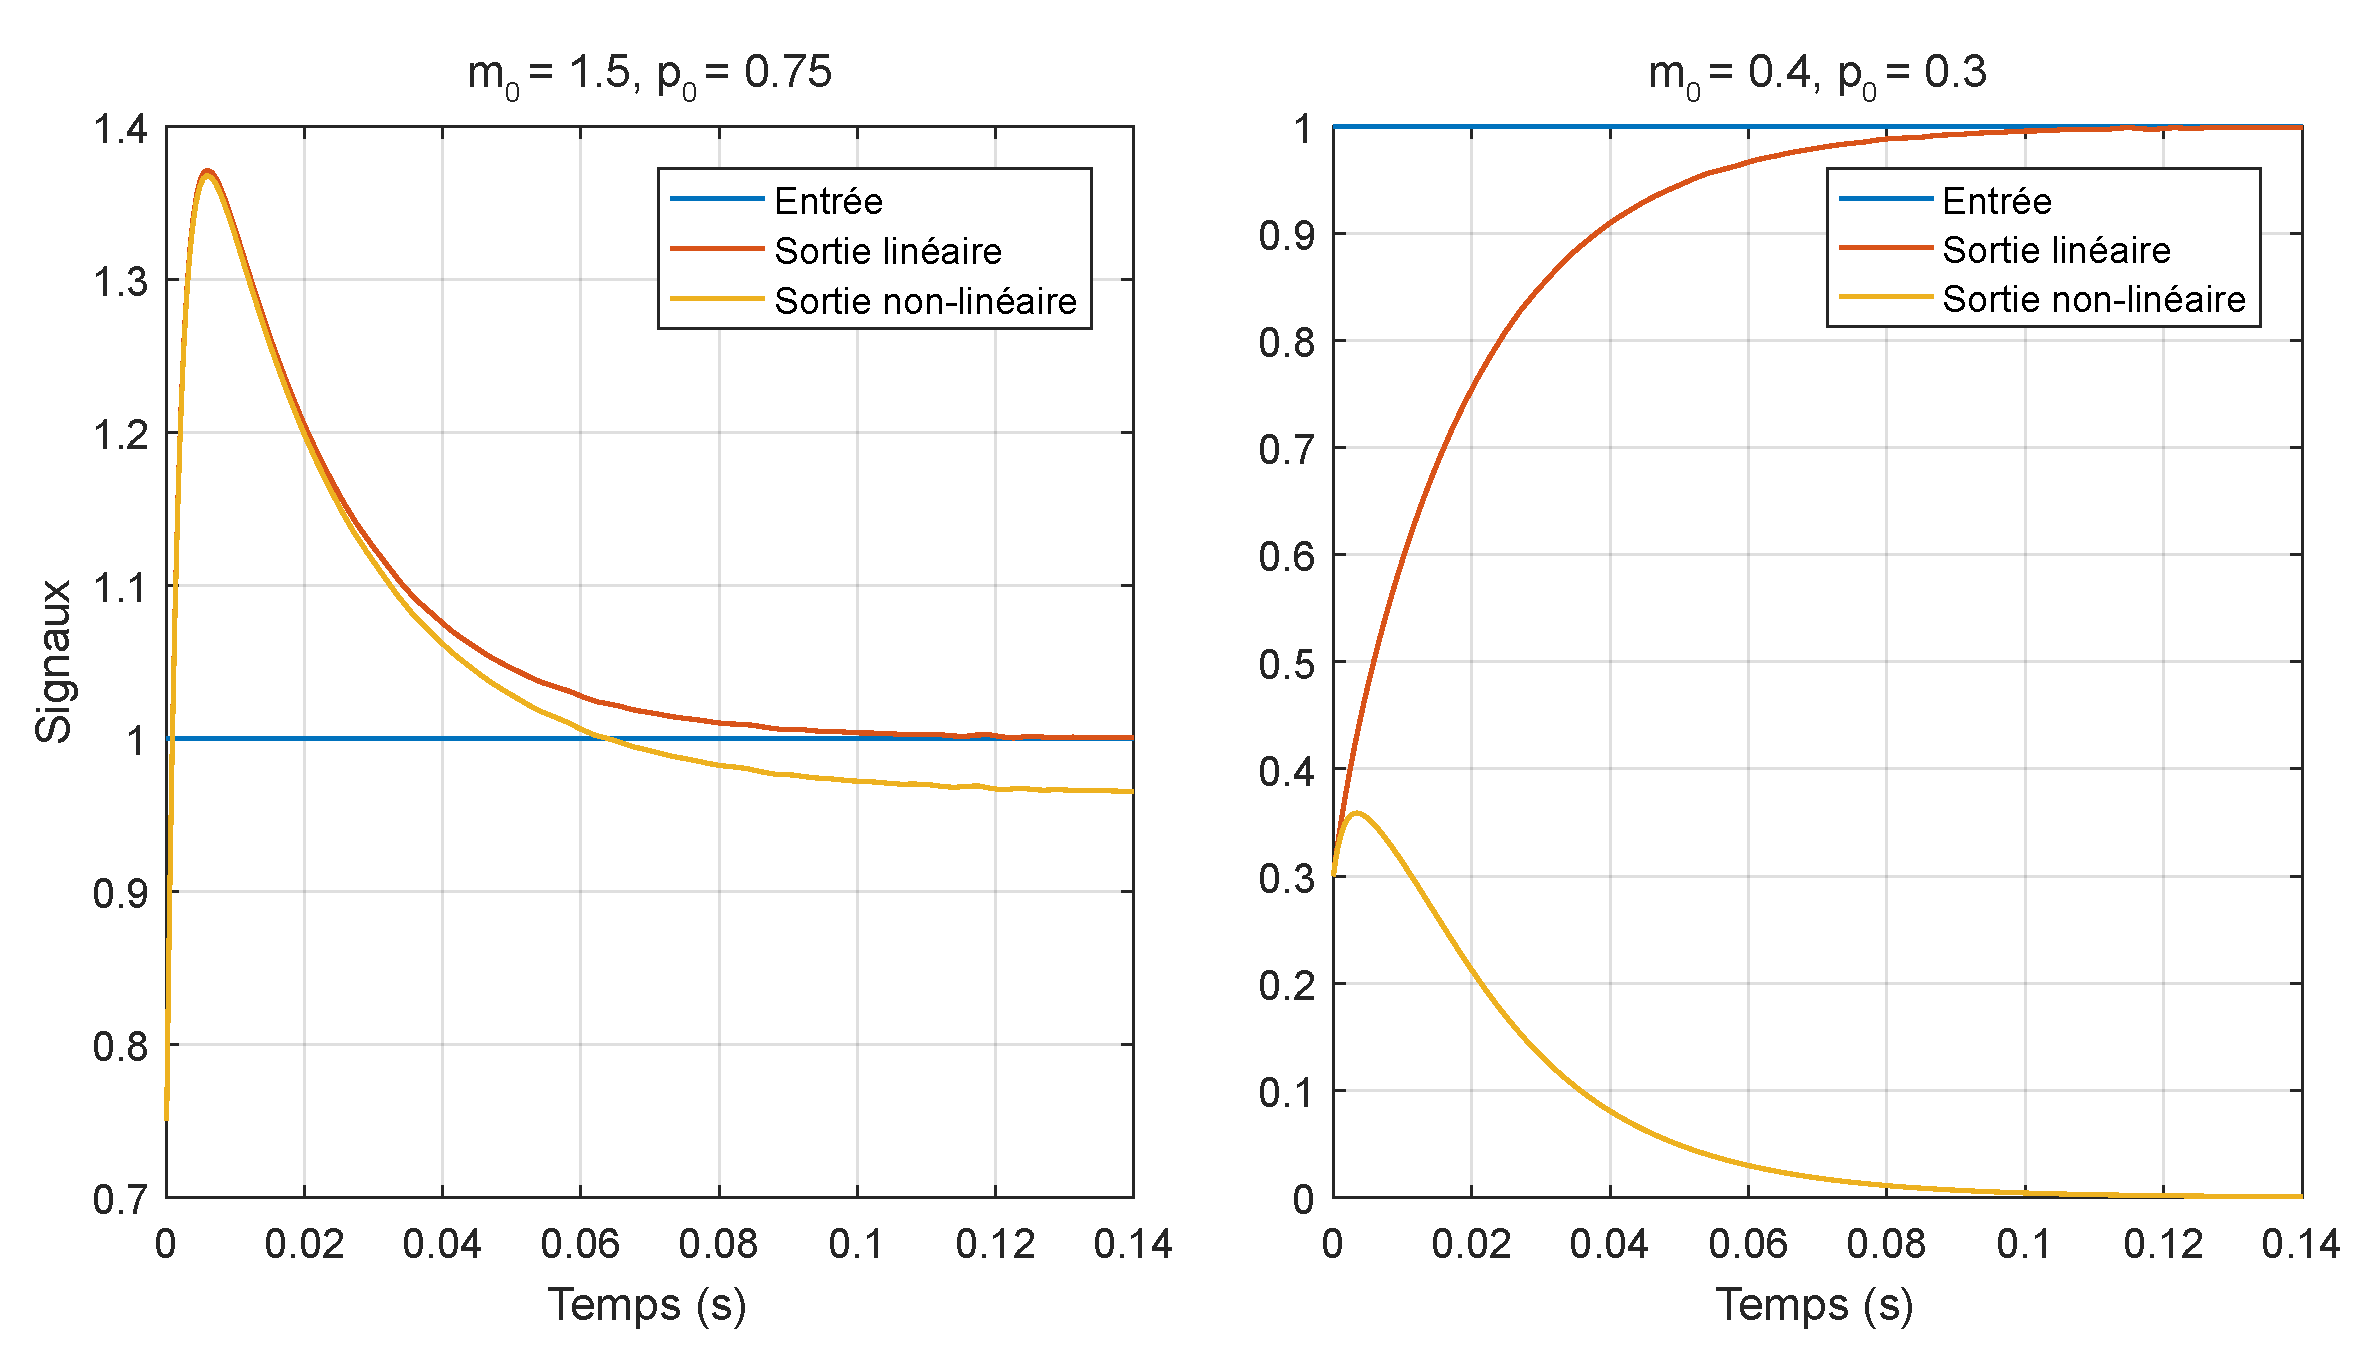
\includegraphics[width = 0.85\textwidth]{resources/pdf/lvsnl.pdf}
		\caption{Comparaison des systèmes linéaire et non-linéaire}
	\end{figure}
	\subsection{Le rôle de l'auto-activation}
	L'auto-activation semble être un mécanisme de régulation permettant à $p$, la concentration en protéines, de rester constante. En effet, même si $p$ chute brusquement suite à une demande importante, puisque $m$, n'étant pas immédiatement touchée par la demande, reste proche de $0.964$, la concentration en protéines reviendra à son état d'équilibre. Néanmoins, si la demande venait à durer, il se pourrait que $m$ ne soit plus suffisante pour \og{} relancer \fg{} le mécanisme.\\\\
	Une demande brusque et importante en protéines pourrait être due, par exemple, à la création d'une nouvelle cellule par mitose ou méiose.
\end{document}